{
\setlength{\parindent}{2em}
\chapter{Methodology}\label{cha:meth}
Like any other project of its size, planning played an important part in this work's good completion. As the present thesis was made in the context of an internship at \gls{MDA}, its development had a lot to gain by adapting to the Dream Chaser team's development process. In addition, because the snapshot feature was a deliverable to the client (\gls{SNC}), it had to adhere as much as possible to certain guidelines, especially concerning deadlines and iterative feedback. Nonetheless, plenty of space was given for creativity and a methodology was adapted to work in parallel with the team. 

\section{Work on the DCCS}
First, the context had to be described, so that a methodology could be devised, both in the team development environment and the personal, more technical part.

\subsection*{Project Management}
The Dream Chaser team was composed of multiple teams handling different aspects of the \gls{BBP}. There were two software and one hardware teams, all of them overseen by the project management team. Most of the work as part of this thesis was done under one of the software teams, counting 10 members. And like many software teams choose to operate, the preferred development method was \textbf{Scrum}. 

Scrum is a very popular agile framework for all types of technical projects all around the world. It allows for a structured, well-defined development and delivery process for relatively small teams part of a complex product \cite{book:scrum}. The main goal of Scrum's usage in the Dream Chaser team was to effectively address its complex engineering problems while creating value for the product (the BBP and its embedded software) and adapting swiftly to unforeseen events during the project. A summary the important concepts of the development process is pictured in \autoref{fig:scrum-process}.

Following the framework's principles, the work of the software team was guided iteratively, using sprints. Their duration was set to two weeks from the start of the Dream Chaser project. This meant that every two weeks, the team took usually half a day to organize the next two weeks for each of its members. In particular, future collaborative work could be coordinated and work units ("stories") could be distributed from the backlog to the members during these "Sprint Review and Planning" meetings.

\begin{figure}[H]
	\centering
	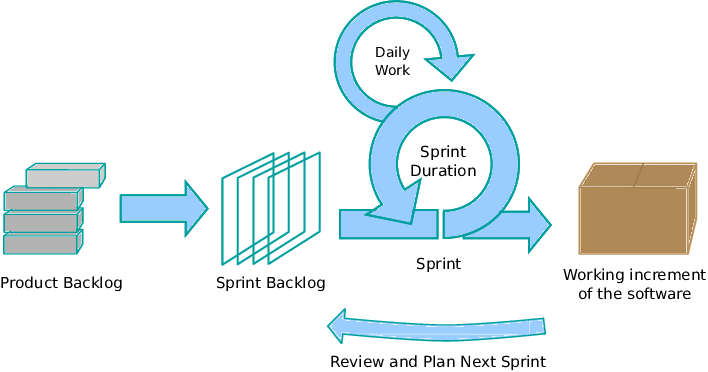
\includegraphics[width=0.9\linewidth,keepaspectratio]{art/scrum-process.png}
	\caption{The Traditional Scrum Life-cycle\cite{misc:scrum-process}}
	\label{fig:scrum-process}
\end{figure}

On top of these organization efforts, the team held 15-minutes meetings everyday, during which each member told the others what they had worked on in the past hours, raised up possible present or future blockers and mentioned the content of their pending work. These daily meetings allowed the team to stay productive, while quickly addressing any arising technical or organizational issues.

\subsection*{Integration of the Thesis Work in Scrum}
Of course, it was very important for this work to fit in the team's development scheme. After all, any project of comparable size needs a work structure and the fact that the team already had a well-working one meant it was an opportunity to adapt the academic project to a working-environment structure. Thus, this avenue was taken from the beginning of the thesis-internship.

Modifying the working method to make it \textit{scrum-able} turned out to have important benefits. For instance, rather than touching base only once in a while during the implementation phase, an update on the progress of the feature had to be given daily to the team. This way, they were able to get daily feedback on the progress of the save \& restore and could quickly provide support if needed. Such a situation happened on many occasions and a lot of time was saved by other members helping with rather technical questions or with finding relevant documentation. 

The daily meetings also brought the thesis subject "closer" to the team. Since the feature was linked to a customer requirement, it was critical for the team leader to have good insights on the overall progression and the predicted release date. A backlog of remaining stories linked to the feature had to be maintained for the team leader to be constantly up-to-date on the progression. Undoubtedly, knowing what to expect in the short and long term is always a big benefit for any project's organization. 

On top of everything, merging the thesis into the Scrum framework also allowed for a much better social integration and better working experience as a whole. 

\section{Breakdown into phases}
The save \& restore function in \gls{BBPSim} is a boolean feature: either it works and the simulator can consistently restart itself back to a previous state, or it doesn't. Like any other program, \gls{BBPSim} needs all of its components to function correctly. Therefore, partial saves of a simulation would lead to stability issues when restoring. 
In any case, such a binary feature should never be entirely programmed without incremental testing, because reverting back the strategy in the event of a failure would be too time-consuming.

This is why the thesis was broken down into phases, where each phase was considered done when it hit a certain milestone at the end. The milestones were chosen so that a save and a restore operation could be successfully done on one component or group of components in the simulator. In addition, in order to adapt the development of the feature to the Scrum framework, each phase was further divided into Scrum stories. That way, it was possible to estimate the time of completion of a certain milestone, since all stories in Scrum are subject to a time estimation before getting assigned. \autoref{tbl:project-phases} better shows how the thesis was divided. Since \gls{BBPSim} was a software with clearly defined layers, it was decided to fit the phases onto them.

This particular division of tasks was chosen, because most of the milestones also made the holding of demonstrations to stakeholders possible. Since this feature was part of a release of the simulator, \autoref{sec:feedback} further explains how the interaction with interested parties was handled.

\begin{table}[htbp]
	\centering
	\ra{1.2}
	\begin{tabularx}{\linewidth}{c X}
	\toprule
	\textbf{Phase} & \textbf{Milestone}\\
	\midrule
	1 & {Access to \gls{FSW} variables}\\
	2 & {Choice of state file format}\\
	3 & {Well-defined mechanism for restoring from file}\\
	4 & {\gls{DAS} memory layer saved \& restored}\\	
	5 & {Shared Memory layer saved \& restored}\\
	6 & {\gls{BBPSim} OS layer saved \& restored}\\
	7 & {\gls{BBPSim} Hardware layer saved \& restored}\\
	8 & {\gls{DAS} execution saved \& restored}\\
	\cmidrule{2-2} 
	-  & \textbf{Stable save \& restore}\\
	\cmidrule{2-2} 
	9 & {Snapshot of file system}\\
	10 & {Verification \& Validation integration}\\
	\cmidrule{2-2} 
	- & \textbf{Feature delivery}\\
	\bottomrule
	\end{tabularx}
	\caption{Division of the thesis work into phases and their milestone.}
	\label{tbl:project-phases}
\end{table}

\section{Customer and Internal Feedback}\label{sec:feedback}
As mentioned previously, this thesis was divided into phases, so that it would be possible to clearly keep track of the progress. However, the division was motivated by the ability to deliver periodic updates not only to the management team, but also to the customer.

As a contractor in the space sector, \gls{MDA} has everything to gain by having good commercial relationships with its customers. This is why meetings with \gls{SNC} were held during this project. Their main goal was to improve transparency with the client, but they were also used to gather important feedback to iterate over the feature's implementation details. 

As for internal feedback, sessions were also held every three to four weeks with members of the software and management teams. Their purpose was to demonstrate the evolution of the feature to stakeholders. As a side effect, this made the thesis "Proof-of-Concept-driven", because progress was motivated by getting the product demo-ready.
}